% chapter 2: Radiation Therapy with Photons

\section{Energy loss of photons in matter}
\begin{figure}[hbt]
\centering
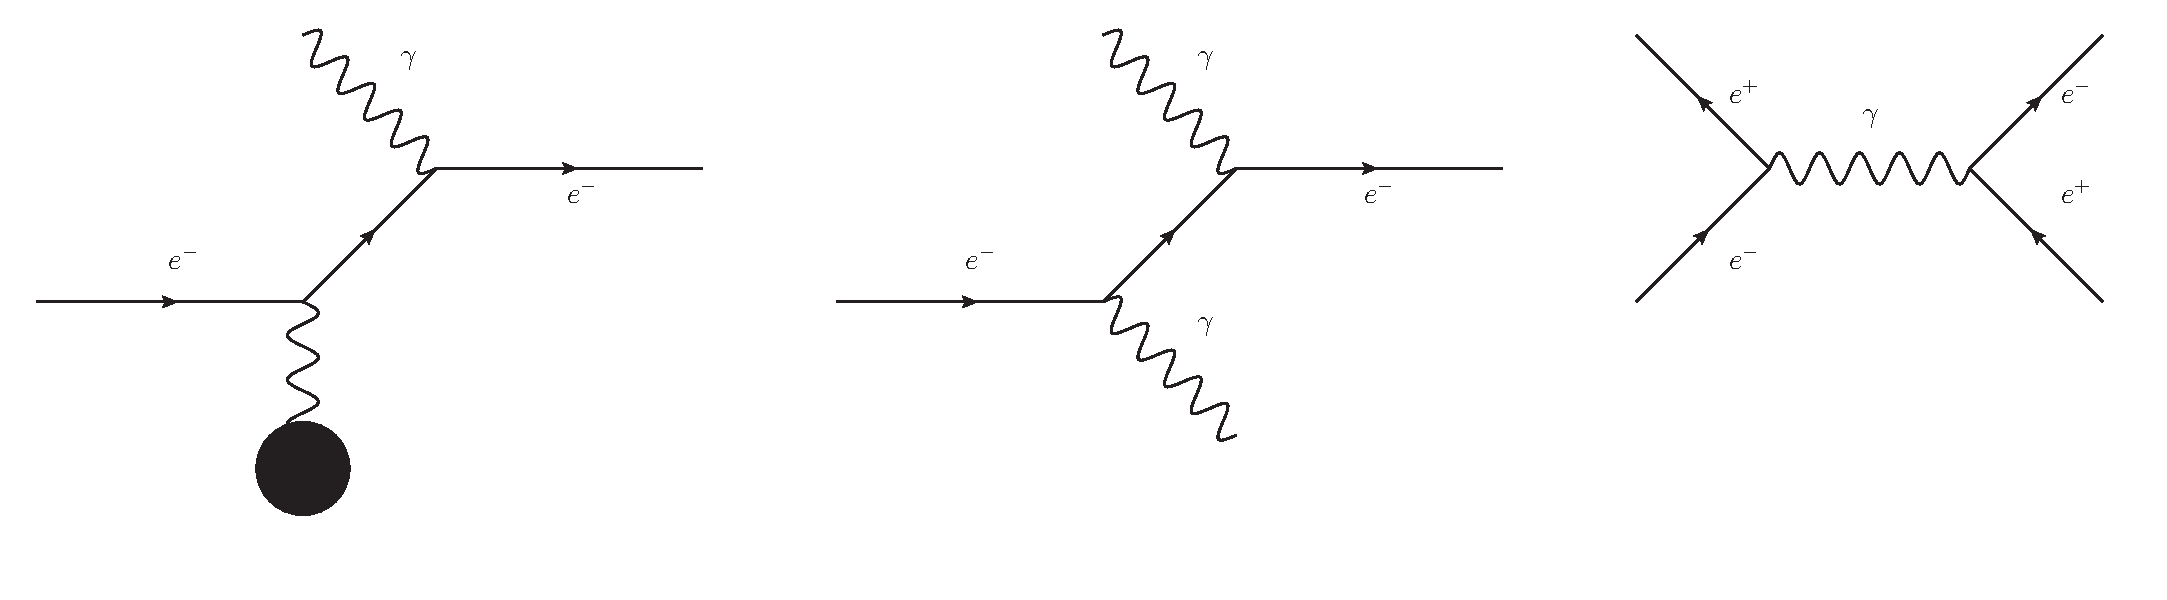
\includegraphics[scale = 0.42]{/Users/alex/Master/contents/images/feynmangraphs.eps}
\caption{Overview on the physical effect responsible for the energy loss of photons in matter. Photoelectric effect (left), Compton effect (middle) and Pair production (right).}
\label{fig:feynmangraphs}
\end{figure}
In particle physics, the photon ($\gamma$) is the mediator for the electromagnetic force. It is neutral and has zero mass. The latter is by virtue of the gauge invariance of the photon field's Lagrange function in quantum field theory. The photon moves with the speed of light $c \approx 3\times10^8$ m/s. Since it is electrically neutral, it will not lose energy via the Coulomb force when interacting with matter. Instead, photons will travel a particular distance before being annihilated. The energy transfer of photons to matter is a combination of three different physical effects: Photoelectric effect, Compton scattering and Pair production (cf. figure \ref{fig:feynmangraphs}). All of them are involved in the gradual energy loss of the photon, but are dependent on the initial energy and material that the photon is passing through. The distance travelled by a photon in matter is governed by a statistical process depending on a linear attenuation coefficient $\mu$, describing the probability of the matter penetration by the photon. All three effects have a contribution to its total travelling distance.
\begin{equation}
\mu = \tau + \sigma + \kappa
\end{equation}
If electromagnetic radiation with incident intensity $I_0$ travels through a material with absorption coefficient $\mu$ and dimension $x$, the intensity at $x$ is
\begin{equation}
I = I_0 \exp(-\mu x).
\end{equation}

\subsection{Photoelectric effect}
The photoelectric effect describes the emission of electrons from matter as a consequence of the absorption of a photon. This emission occurs only if the incident photon energy is larger than the binding energy of electron in the atom. In this case the photon is completely absorbed and the electron is emitted. If the photon energy is too low, the electron will not be able to escape the material as a photoelectron. After its emission, the photoelectron has the following energy
\begin{equation}
E_e = h\nu - E_b,
\end{equation}
where $h$ is Planck's  constant $h = 6.626068 \times 10^{-34}$ m$^2$kg/s, $\nu$ the frequency of the incident photon and $E_b$ the binding energy of the electron within the atom. The photoelectric effect is dominant in the low energy regime within a few hundred keV. When a photoelectron is extracted, the corresponding absorber atom becomes ionized. The created vacancy is filled by an upper shell electron, which can generate characteristic X-ray photons. In some cases this process will emit an Auger electron instead of a photon.\\The contribution of the photoelectric effect to the linear attenuation coefficient $\mu$ is represented by the photoelectric absorption coefficient $\tau$. It is highly dependent on the atomic number $Z$ \cite{Bethge}
\begin{equation}
\tau = \left(\frac{32}{E^7}\right)^{1/2}\alpha^4Z^n\underbrace{\left(\frac{8}{3}\pi r_e^2\right)}_{\sigma_\mathrm{Th}}\hspace{1cm}\mathrm{with}\hspace{1cm}n\in [4,5].
\end{equation}
Here $\alpha=1/137$ is the electromagnetic coupling constant and $\sigma_\mathrm{Th}$ the Thomson cross section for elastic scattering. For materials with lower atomic numbers $\tau$ is proportional to $Z^4$. If the atomic number $Z$ is larger than 10, then $\tau \propto Z^5$.

\subsection{Compton scattering}
The Compton effect describes the scattering of a recoil electron by an incident photon. The photon is deflected through an angle $\theta$ with respect to its incident direction. In contrast to the photon from the photoelectric effect, the probability of the Compton effect occurring increases with incident photon energy.. A portion of this energy is transferred to the electron, which is assumed to be initially at rest. The scattered electron is called a recoil or Compton electron. The portion of energy that can be transferred to the Compton electron can vary from zero up to $E=0.8 E_\gamma$ of the incident photon energy $E_\gamma$. The energy of the the scattered photon can be derived by equating the four-momentum vectors of the incident photon $\mathbf{p}_\gamma$, electron at rest $\mathbf{p}_e$, scattered photon $\mathbf{p}_{\gamma^\prime}$ and Compton electron $\mathbf{p}_{e^\prime}$. The scattered photon then has the energy
\begin{equation}
E_{\gamma^\prime} = \frac{E_\gamma}{1+\frac{E_\gamma}{m_ec^2}(1-\cos\theta)}.
\end{equation}
By introducing the Compton wavelength $\lambda_C = h/m_ec \approx 0.0243\times 10^{-10}$m the change in wavelength is
\begin{equation}
\Delta \lambda = \lambda_C(1-\cos\theta)
\end{equation}
The contribution of the Compton effect to the total linear attenuation coefficient $\mu$ can be calculated by deriving the Compton cross section \cite{Jauch}
\begin{equation}\label{eq:comptoncrosssection}
\sigma = \frac{\pi r_e^2}{E} \left[4+\frac{2E^2(1+E)}{(1+2E)^2}+\frac{E^2-2E-2}{E}\ln(2+2E)\right].
\end{equation}
Here $r_E$ is the classical electron radius $r_E = e^2/m_ec^2 = 2.82\times 10^{-15}$m and $E$ the energy of the incident photon divided by the rest energy of the electron $m_ec^2$. The Compton cross section has two special cases, called the Thomson and Klein-Nishina regimes. The case $E/mc^2 \ll 1$ is defined as the Thomson regime, while $E/mc^2 \gg 1$ is described by the Klein-Nishina regime. Both regimes are part of the asymptotic behaviour of eq. \ref{eq:comptoncrosssection} \cite{Heitler}:
\begin{equation}
\sigma \rightarrow\begin{cases}
\frac{8\pi r_e^2}{3}\left[1-2E+\frac{26}{5}E^2+O(E^3)\right]\hspace{1cm}\mathrm{for}\hspace{1cm}E\ll 1\\
\frac{\pi r_e^2}{E}\left[\ln(2E)+\frac{1}{2}+O(E^{-1})\right]\hspace{1.57cm}\mathrm{for}\hspace{1cm}E\gg 1.
\end{cases}
\end{equation}
The higher the energy of the incident photon, the more energy is transferred to the recoil electron. In total the recoil electron receives the largest portion of energy from the photon in the lowest energy region. The Compton effect is dominant in the regime of a few MeV.

\subsection{Pair production}
As soon as the incident photon energy exceed double the mass of an electron $2m_e = 1.022$ MeV, pair production becomes possible. This effect occurs when the photon interacts with a heavy nucleus. The incident photon disappears and a positron electron pair is produced
\begin{equation}
\gamma \rightarrow e^+ + e^-.
\end{equation}
Depending on the energy of the photon, both the electron and the positron will have kinetic energy to travel through matter around them. The positron normally travels a small distance until it interacts with another electron. In this interaction both particles are annihilated and two photons are created. The cross section for pair production can be extremely complicated if all occurring phenomenons are included, especially Coulomb, screening and radiative corrections. For radiation therapy it is sufficient to assume an increasing cross section $\kappa$ for larger photon energies $E$. The differential cross section is represented by the corrected Bethe-Heitler formula
\begin{equation}
\begin{split}
\frac{\mathrm{d}\sigma(Z,\varepsilon)}{\mathrm{d}\varepsilon} = & \alpha r_e^2 Z \left[ Z + \xi(Z) \right] \left( \left[ \varepsilon^2 + \left(1 - \varepsilon \right)^2 \left[ \Phi_1(\delta(\varepsilon)) - \frac{F(Z)}{2}\right] \right]\right.  \\
& \left.+ \frac{2}{3} \varepsilon \left(\varepsilon\right) \left[\Phi_2(\delta(\varepsilon)) - \frac{F(Z)}{2} \right] \right)
\end{split}
\end{equation}
where $\varepsilon=E/E_\gamma$ with $E$ being the total energy carried away by the electron-positron pair and $E_\gamma$ the energy of the incident photon. The functions $\Phi_i$ and $F(Z)$ are parametrized functions for the screening effect of the electromagnetic field depending on the screening variable $\delta(\varepsilon)$. For small energies in medical physics, it is sufficient to assume a linear proportionality to the cross section
\begin{equation}
\tau\propto E
\end{equation}
Pair production becomes dominant if the energy of the incident photons is 10 MeV and higher.

\subsection{Combined cross section for photons in matter}
\begin{figure}[htp]
\centering
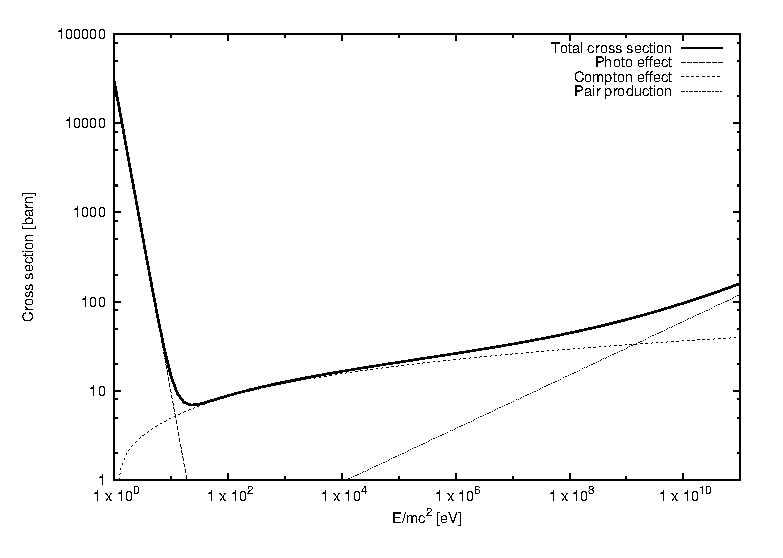
\includegraphics{/Users/alex/Master/contents/images/photonxsec.eps}
\caption{Total cross section $\mu$ in units of barn (10$^{-28}$m$^2$) in the region from 1 eV up to 10 GeV. For radiotherapy, the Compton effect is most prevalent, as the common energies are in the range of a few MeV.}
\label{fig:photonxsec}
\end{figure}
Photoelectric effect, Compton scattering and Pair production are dominant for specific energy regions of the incident photon. The photoelectric effect is dominant in the range of a few keV, whereas the Compton effect becomes important at the MeV scale up to 10 MeV. Afterwards pair production becomes the largest contribution for the interaction of photons with matter. Conventional radiation therapy uses energy on a scale of a few MeV, which means that the Compton effect prevails for this application. Figure \ref{fig:photonxsec} shows the total cross section for the photon in the energy regime of 0 MeV up to 10 GeV.
\subsection{Interaction of Charged Particles with Matter}
Charged particles exhibit different behaviours when interacting with matter. Interactions either occur via inelastic scattering with electrons or elastic scattering with a nucleus. Therefore the analytical form of the energy loss per path length is much more complicated, as it can only be computed from quantum electrodynamics. Bethe and Bloch were the first to derive this equation \cite{Leo}
\begin{equation}\label{eq:bethebloch}
- \frac{dE}{dx} = \frac{4 \pi}{m_e c^2} \cdot \frac{nz^2}{\beta^2} \cdot \left(\frac{e^2}{4\pi\varepsilon_0}\right)^2 \cdot \left[\ln \left(\frac{2m_e c^2 \beta^2}{I \cdot (1-\beta^2)}\right) - \beta^2\right].
\end{equation}
The parameters in the Bethe-Bloch formula are defined as follows
\begin{itemize}
\item $\beta = v/c$ with v being the velocity of the particle and $c=3\times 10^8$m/s the speed of light.
\item $E$ energy of the particle.
\item $x$ distance travelled by the particle.
\item $z$,$e$ particle charge in units of an electron charge.
\item $m_e$ rest mass of the electron.
\item $n$ electron density of the target.
\item $I$ mean excitation potential of the target.
\item $\varepsilon_0$ vacuum permittivity of the target material.
\end{itemize}
Charged particles are also able to lose energy via Bremsstrahlung, Cherenkov radiation or nuclear interactions. A simple form of equation \ref{eq:bethebloch} for electrons and positrons can be derived as well \cite{Leo}
\begin{equation}\label{eq:bethe}
- \frac{dE}{dx} = \frac{4 \pi}{m_e c^2} \cdot \frac{nz^2}{\beta^2} \cdot \left(\frac{e^2}{4\pi\varepsilon_0}\right)^2 \cdot \left[\ln\left(\frac{\tau^2(\tau + 2)}{2(I/m_ec^2)^2}\right)+F(\tau)\right].
\end{equation}
$\tau$ is the kinetic energy of the incoming particle measured in units of $m_ec^2$. The function $F(\tau)$ can be calculated for positrons and electrons via an approximation:
\begin{equation}
F(\tau) = \begin{cases}
1 - \beta^2 + \frac{\tau/8 - (2r+1)\ln(2)}{(\tau + 1)^2} & \mathrm{for}~e^-\,\\
2\ln(2) - \frac{\beta^2}{12}\left(23 + \frac{14}{\tau + 2} + \frac{10}{(\tau + 2)^2} + \frac{4}{(\tau + 2)^3}\right)& \mathrm{for }~e^+.
\end{cases}
\end{equation}
For charged particles, the linear energy transfer (LET) defines the energy transferred to a material as the particle travels through it. While equation \ref{eq:bethe} focuses on the energy loss per unit distance traveled by the particle, LET describes the energy transferred to the material surrounding the particle track with due regard to secondary electrons. LET is defined as
\begin{equation}
\mathrm{LET} = \frac{\mathrm{d}E_\Delta}{\mathrm{d}x},
\end{equation}
where $E_\Delta$ is the energy loss due to the collisions of the charged particle with the material minus the kinetic energy of all secondary electrons with energy $E>E_\Delta$. The larger the LET, the more secondary electrons are induced, which creates a larger energy deposition in the material.
\section{Radiation biology of photons}
\subsection{DNA radiation damage}
Biological damage caused by ionizing radiation is closely linked to the damage response of DNA. DNA damage can be quantified by looking at the DNA strand breaks, caused by charged particle tracks. DNA itself is constructed as a double-helix structure consisting of two strands, which are connected by a hydrogen bond. The so called sugar-phosphate group is the 'backbone' of each strand. If a single strand is broken, it does not necessarily lead to cell killing, as the DNA is able to repair itself by using the opposite strand as a template for its repair mechanism. If the repair is incomplete or incorrect, it leads to DNA mutation. In most cases, single-strand breaks (SSB) can either be repaired or lead to mutation due to misrepair. Double-strand breaks (DSB), on the other hand, are more difficult to repair. If a break in two strands is created within a few base pairs of the sugar-phosphate backbone, it creates a DSB. These DSB are one of the main sources for lethal lesions in DNA, since they create cell kill, carcinogenesis or mutation due to DNA misrepair. DSBs can occur either through direct ionization, or free radicals, created by the incident radiation. The charged particle tracks forming DNA strand breaks for photons are usually created by electrons \cite{Alper}. Figure \ref{fig:DNABreaks} shows all different scenarios linked to SSB and DSB induced radiation damage in DNA. 
\begin{figure}[ht]
\centering
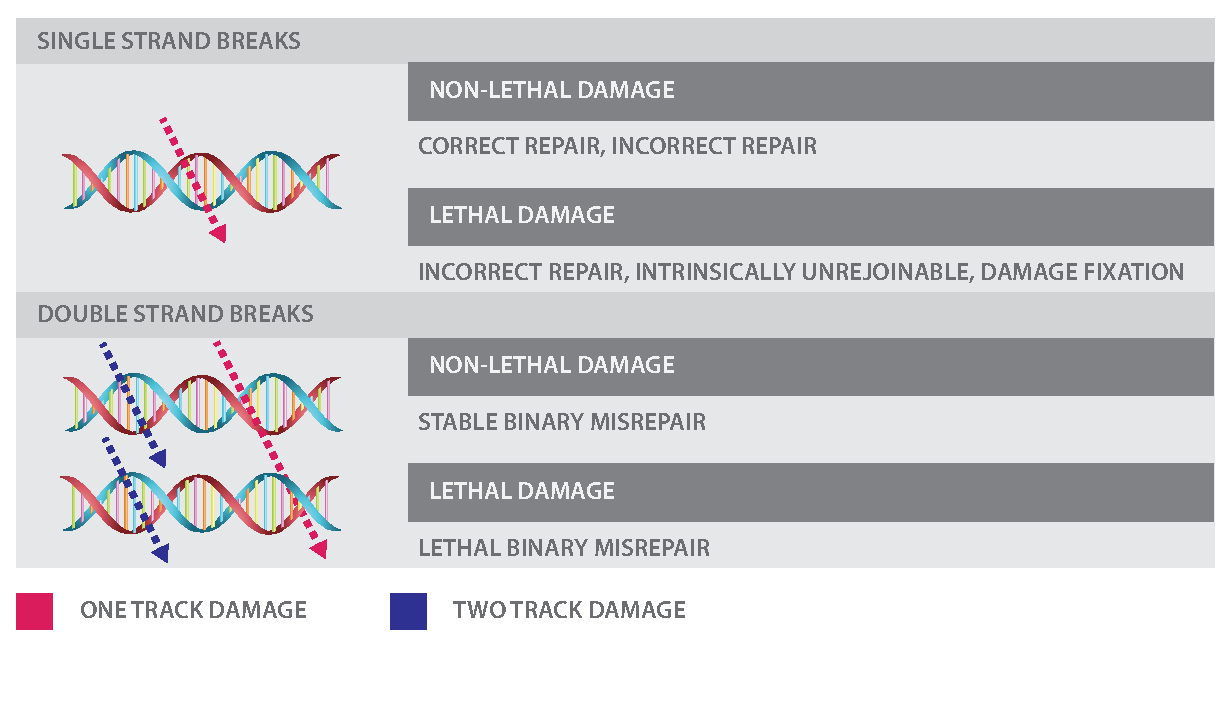
\includegraphics[scale = 0.7]{/Users/alex/Master/contents/images/DNABreaks.eps}
\caption{Damage mechanism of single and double strand breaks in DNA through ionizing radiation. Single stand breaks are only assigned to radiation damage that is created by one particle track, while double stand breaks are generated either by two seperate single tracks or a single track creating single strand breaks in two DNA strands. }
\label{fig:DNABreaks}
\end{figure}
\subsection{The linear-quadratic model}
The linear-quadratic model describes the relation between exchange-type chromosome aberrations resulting from two separate DNA strand breaks and absorbed dose $D$ \cite{Hall}. This model relates an absorbed dose $D$ within a voxel to its biological effect $\varepsilon$. The biological effect $\varepsilon$ can be calculated by combining  the radio response parameters $\alpha_i$ and $\beta_i$ with the absorbed dose $D_i$ in the voxel $i$,
\begin{equation}
\varepsilon_i(D_i) = \alpha_i D_i + G\beta_i D_i.
\end{equation}
Here $G$ is the time dependent Lea-Catcheside dose protraction factor \cite{pmid9343102}, which will be assumed to be $G=1$ for further considerations. The radio response parameters $\alpha$ and $\beta$ are parameterizations of the DNA single and double-stand breaks emerging from radiation damage. The dose $D$, where contributions to cell killing from the linear and quadratic terms are equal is
\begin{equation}
D = \frac{\alpha}{\beta}.
\end{equation}
In the linear quadratic model, radiation damage is categorized into linear and quadratic dose contributions. These contributions are dependent on the tissue that is irradiated. In table \ref{tab:oartissueparameter} and \ref{tab:tumortissueparameter} different $\alpha$ and $\beta$ values are shown.
\begin{table}[htb]
\centering
\footnotesize
\begin{tabular}{llcccc}
\toprule
\multicolumn{3}{c}{Study Information} & \multicolumn{3}{c}{Parameter Data} \\
\cmidrule(r){1-3} \cmidrule(r){4-6}
Study by & Tissue type & $D_{50}$ [Gy]& $\alpha/\beta$ [Gy] & $\alpha$ [Gy$^{-1}$] & $\beta$ [Gy$^{-2}$]\\
\midrule\\
\textit{Cronqvist et al.}\cite{CronqvistThesis}& Brain \& temporal lobes&60 & 2 & 0.062 & 0.031\\
& Brainstem & 65.1 & 2 & 0.062 & 0.031\\
& Chiasm & 65.0 & 2 & 0.0511 & 0.0256\\
& Eyes & 65.0 & 2 & 0.0407 & 0.0203\\
& Larynx & 80.0 & 3 & 0.0281 & 0.0094\\
& Middle-external ears & 65.0 & 3 & 0.0915 & 0.0305\\
& Optical nerves & 65.0 & 2 & 0.0511 & 0.0256\\
& Parotids & 46.0 & 3 & 0.0675 & 0.0225\\
& Spinal Cord & 68.6 & 2 & 0.0407 & 0.0203\\
& Temporomandibular joints & 70.3 & 3 & 0.0918 & 0.0306\\
& Trachea-esophagus & 68.0 & 3 & 0.0708 & 0.0236\\\\
\textit{Eisbruch et al.}\cite{pmid10524409}& Parotids & 28.4 & 3 & 0.13 & 0.0433\\\\
\textit{Honore et al.}\cite{pmid12413669}& Inner ears & 50.0 & 3 & 0.0265 & 0.0088\\\\
\textit{Roesink et al.}\cite{pmid11704314}& Parotids & 39.0 &3 & 0.0413 & 0.0138\\\\
\textit{Schultheiss et al.}\cite{pmid18243570}& Spinal Cord & 68.6 &0.87 & 0.0577 & 0.0663\\\\
\textit{Withers et al.}\cite{pmid7836089}& Subclinical disease & 27.0 & 10 & 0.0554 & 0.0055\\\\
\bottomrule\\
\end{tabular}
\caption{Tissue parameters for organs at risk derived from various studies. }
\label{tab:oartissueparameter}
\end{table}
\begin{table}[tbh]
\centering
\small
\begin{tabular}{llcccc}
\toprule
\multicolumn{2}{c}{Study Information} & \multicolumn{3}{c}{Parameter Data} \\
\cmidrule(r){1-2} \cmidrule(r){3-5}
Study by & Tissue type/cell & $\alpha/\beta$ [Gy] & $\alpha$ [Gy$^{-1}$] & $\beta$ [Gy$^{-2}$]\\
\midrule\\
\textit{Carlson et al.}\cite{pmid18363426}& Prostate & 3.1 & 0.15 & 0.048\\\\
\textit{Cronqvist et al.}\cite{CronqvistThesis}& Nasoph. cancer T1 \& T2 & 10 & 0.1124 & 0.0112\\
& Nasoph. cancer T3 \& T4 &10 & 0.0854 & 0.0085\\\\
\textit{Furusawa et al.}\cite{pmid11025645}& HSG & 5.1 & 0.313 & 0.184\\
& T1 &0.52 & 0.0305 & 0.0585\\
& V79 &9.2 & 0.184 & 0.02\\\\
\textit{Kraemer et al.}\cite{pmid11098906}& Chordoma & 2 & 0.1 & 0.05\\\\
\textit{Stuschke et al.}\cite{pmid10435801}& Head \& Neck & 10 & 0.25 & 0.025\\\\
\textit{Withers et al.}\cite{pmid7836089}& Subclinical disease & 10 & 0.0554 & 0.0055\\\\
\bottomrule\\
\end{tabular}
\caption{Tissue parameters for tumor tissue derived from various studies.}
\label{tab:tumortissueparameter}
\end{table}
The biological effect $\varepsilon$ can be related to the survival fraction of clonogens after being irradiated with dose $D$.
\begin{equation}
S(D) = \exp(-\varepsilon) = \exp(-(\alpha D + \beta D^2)).
\end{equation}
Therefore $\varepsilon$ can be interpreted as the expected number of lethal lesions per cell, when irradiating the cell with dose $D$. When the initial number of tumour clonogens $N$ is known, the tumour control probability (TCP) can be calculated:
\begin{equation}
\mathrm{TCP} = \exp(-N\cdot S(D)å) = \exp\left(-Ne^{-(\alpha D + \beta D^2)}\right).
\end{equation}
TCP relates tumour size and radiation dose to the probability of local tumour control.
\subsection{Oxygen effect}
Oxygen has been found to be one of the most important pharmacological agents that is able to alter the biological effect of ionizing radiation \cite{petry} \cite{mottram} \cite{pmid13106296}. The tumour vasculature can be distorted, which can frequently lead to hypoxic regions which demand a higher dose to achieve the same radiation damage as under fully oxygenated conditions. The ratio of dose administered under hypoxic to fully oxygenated conditions needed to achieve the same biological effect is called oxygen enhancement ratio (OER).
\begin{equation} 
\mathrm{OER} = \frac{D_{\mathrm{Hypoxic}}}{D_{\mathrm{Aerobic}}}.
\end{equation} 
For photons, in vitro OER values have been measured between 2.5 - 3.5 \cite{Hall}. In general the higher efficiency of radiation damage in highly oxygenated regions of the tumour has been affiliated with the \textit{oxygen fixation hypothesis}. When DNA is damaged by ionizing radiation it can be chemically seen as a DNA radical (DNA$\cdot$). The DNA$\cdot$ radical will either react with an SH group to DNA-H, leading to chemical restitution, or with molecular O$_2$. The latter leads to the formation of a DNA-OO$\cdot$ radical, which then combines with another hydrogen to DNA-OOH. The damage fixation caused by a unrejoinable DSBs leads to cell death. In general the mechanism of the oxygen fixation hypothesis has a half-life of 10$^{-10}$s for ion pairs and 10$^{-5}$s for free radicals, which demands the the presence of oxygen in this timeframe after the interaction with incident radiation. Oxygen in tissue is generally bound in water H$_2$O. When photons interact with this compound, the following reaction is initialized
\begin{equation}
\gamma + \mathrm{H}_2\mathrm{O}\rightarrow \mathrm{H}_2\mathrm{O}^+ + e^- \xrightarrow{\mathrm{H}_2\mathrm{O}} \mathrm{H}\cdot +\mathrm{H}_3\mathrm{O}^++\mathrm{OH}\cdot
\end{equation}
The OH$\cdot$ can either recombine with another OH$\cdot$ to for hydrogen peroxide (H$_2$O$_2$), or with a DNA radical to form a non-reversable organic peroxide RO$_2\cdot$. This leads to a non-repairable state of the DNA radical, causing cell death. Therefore, abundance of oxygen leads to a chemical change in the radiation damage formed in the DNA. These reactions are limited, if tumour regions are hypoxic, yielding in a higher probability of DNA repair and recovery. The presence of oxygen 'fixes' (hence \textit{fixation hypothesis}) the damage done by free radicals, creating permanent lesions leading to cell killing, carcinogenesis or mutation (which also can lead to lethal damage).\\This mechanism leads to a connection between hypoxia and poor outcomes of radiation therapy. The OER has been shown to increase with higher oxygen partial pressures with a half maximum OER at 3 mmHg or 0.5\% oxygen \cite{ pmid15183486}. In general OER is affected by the nature of cellular radio sensitivity, incident radiation, oxygen tension in the considered volume, time of oxygen presence and the cell cycle, as the S-phase is more resistant.
\subsection{Origin of hypoxia in tumours}\label{chap:hypoxiaorigin}
\begin{figure}[tb]
\centering
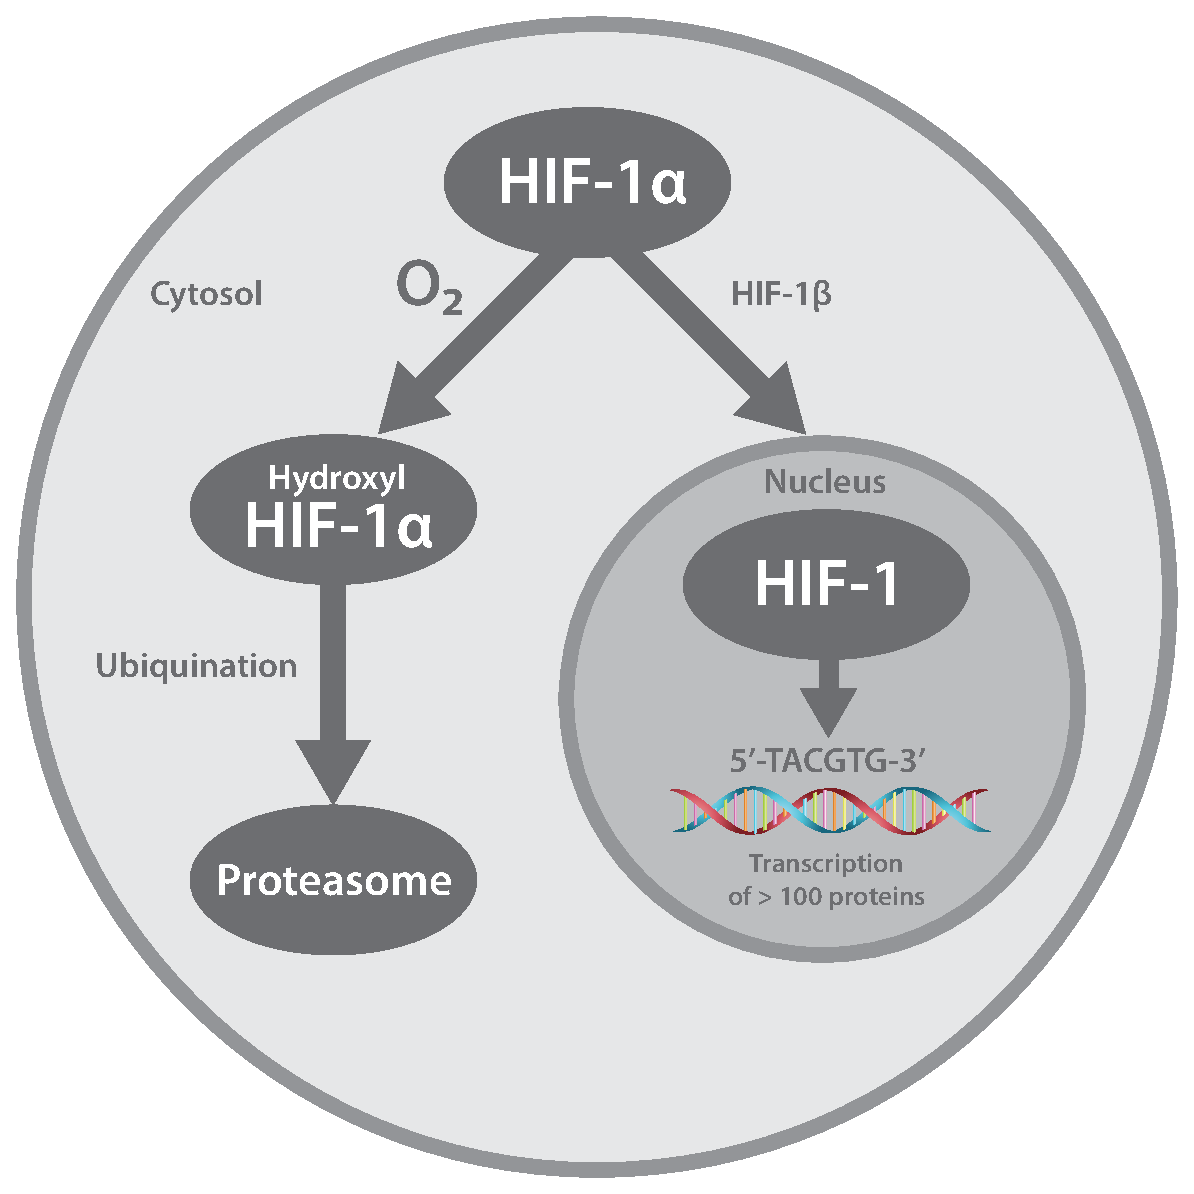
\includegraphics[scale = 0.4]{/Users/alex/Master/contents/images/HIFAlpha.eps}
\caption{HIF-1$\alpha$ mechanism for the transcription of proteins in DNA that increase cell survival in tumour cells in hypoxic environments.}
\label{fig:HIFAlpha}
\end{figure}
A healthy cell in normal tissue which is deprived of oxygen will die. Tumour cells on the other hand are generally exposed to chronic hypoxia as their growth will lead to lack of vasculature to supply inner regions with enough oxygen. Lack of oxygen can then lead to decreased radiation response and to an underestimated cell kill. This is also true for chemotherapy as the poor perfusion can lead to limited access to certain tumour areas. The underlying biochemistry of hypoxia in tumours has become more and more complex with the appearance of accurate description of transcription factors. For hypoxia the \textit{hypoxia inducible factor 1} (HIF-1) is the transcriptions factor that leads to the higher cell survival. This is achieved by up-regulating more than 100 proteins that promote survival and especially the aggressiveness of the hypoxic tumour cells. The mechanism for HIF-1 in hypoxic and oxic conditions can be described as follows \cite{pmid13130303}:
\begin{itemize}
\item \textit{Oxic conditions: }If oxygen is present with HIF-1$\alpha$, it becomes a hydroxyl. Afterwards it is transformed to a proteasome (regulator for protein concentration and degradation of misfolded proteins) via ubiquitination. 
\item \textit{Hypoxic conditions: } If oxygen is absent, HIF-1$\alpha$ will transform into HIF-1$\beta$. This is accomplished by the translocation of HIF-1$\alpha$ to the nucleus. HIF-1 is the heterodimer (complex of a nucleic acid and a protein) of HIF-1$\beta$, which is the transcription factor for more than 100 hypoxia response elements on the chromosomes. All elements share a specific sequence (5$^\prime$-TACGTG-3$^\prime$) that will activate more than 100 proteins supporting cell survival.
\end{itemize}
Figure \ref{fig:HIFAlpha} shows a detailed schematic description of the HIF-1 mechanism for increased cell survival of tumour cells in hypoxic environments. Hypoxia can occur in two different forms: Chronic and acute hypoxia. Chronic hypoxia is a consequence of oxygen consumption by tumour cells that are inadequately perfused due to the distance between the cancer cells and the nearest blood vessels. Acute hypoxia is the result of the temporary closing of blood vessels due to the malformed vasculature of the tumour \cite{Simon}. Both hypoxia types contribute to general tumour hypoxia and the poor outcome of radio treatment. One of the major differences between these two hypoxia categories, is their time scale variance. While acute hypoxia will show larger fluctuations, chronic hypoxia is more stable. As both hypoxia types possess HIF-1 as its transcription factor, hypoxia tracers are not able to distinguish between them. A mathematical approach to a differentiation of acute and chronic hypoxia is discussed in chapter \ref{chapt:chronicacute}.
\subsection{Impact of hypoxia on cell survival}
Hypoxia will decrease the radio sensitivity of tumour cells. In terms of the linear quadratic survival model, this decrease affects the radio response parameters $\alpha$ and $\beta$. \textit{Carlson et al.} \cite{pmid17022202} introduced a method to incorporate the impact of hypoxia into the linear quadratic cell survival model by using only a single parameter. The number of cells, surviving after being irradiated with a dose $D$ under aerobic conditions is
\begin{equation}
S(D) = \exp\left(\frac{\alpha_A}{\mathrm{HRF}}D + \frac{\beta_A}{\mathrm{HRF}^2}D^2\right).
\end{equation}
Here $\alpha_A$ and $\beta_A$ are radio sensitivity parameters under aerobic conditions. For low-LET radiation, $\alpha$ represents the quantity of lethally misrepaired and unrepaired double-strand breaks, and $\beta$ represents the quantity of lethal exchange-type chromosome aberrations formed through binary misrepair of two separate DSBs \cite{pmid18363426}. As this work is using photon beams for treatment planning, $\alpha_A$ and $\beta_A$ are assumed to be the radio response parameters for photons $\alpha_X$ and $\beta_X$. HRF is the hypoxia reduction factor, which a derived quantity from the current oxygen conditions in a voxel \cite{pmid21183291}.
\begin{equation}\label{eq:hrfmodel}
\mathrm{HRF} = \frac{Km + p}{K+p}
\end{equation}
The functional form of HRF resembles a sigmoidal shape as it describes the clinical data best. The two parameters driving the transformation of oxygen partial pressure values $p$ are $m$, the maximum HRF and $K$, which can be interpreted by inserting $p=K$ yielding HRF = $(m+1)/2$. The HRF concept is equal to an approach used by \textit{Toma-Dasu et al.} \cite{pmid21871003} using the OER. In general the distribution of oxygen partial pressure $p$ in tumour cells is a diffusional process and is dependent on the distance to the capillary wall $p(r)$ \cite{pmid5067983}.
\begin{table}[tb]
\small
\centering
\begin{tabular}{ccccc}
\toprule
\multicolumn{1}{c}{} & \multicolumn{2}{c}{Parameter Data} \\
\cmidrule(r){2-3}
Study by &  $m$ & $K$ [mmHg] & Comment\\
\midrule\\
\textit{Carlson et al.}\cite{pmid21183291}$^\#$ & 2.78 $\pm$ 0.06 & 1.47 $\pm$ 0.14 & \textit{cf.} \cite{pmid7410133}\cite{pmid6718689}\cite{pmid412319}\cite{pmid17022202}\\\\
\textit{Cullen et al.}\cite{pmid4616914}$^*$	 & 2.79 $\pm$ 0.20 & 3.27 $\pm$ 0.35 & \textit{in vivo (attached)}\\
									 & 3.04 $\pm$ 0.13 & 6.16 $\pm$ 0.76 & \textit{in vitro (attached)}\\\\
\textit{Cullen et al.}\cite{pmid1084867}$^*$	 & 2.78 $\pm$ 0.25 & 1.98 $\pm$ 0.49 & \textit{in vivo (suspension)}\\
									 & 2.82 $\pm$ 0.15 & 4.03 $\pm$ 0.61 & \textit{in vitro (suspension)}\\\\
\textit{Wouters et al.}\cite{pmid9146699}$^\&$  & 2.5 ($\alpha$)/3.0 ($\beta$) & 3.28 & \textit{cf.} \cite{pmid412319}\cite{pmid6718689}\\\\
\bottomrule\\
\textbf{Combined} & 2.82 $\pm$ 0.05 & 1.94 $\pm$ 0.13 & 
\end{tabular}
\caption{Model parameters from different in vivo and in vitro studies. All studies used photons as radiation source to derive parameter data. Remarks: $^*$Ehrlich ascites tumor cells, $^\#$ Values and error recalculated from original data and fit, $^\&$ not included in combined value since no error was available. Error from the \textit{Carlson et al.} was not available in the published article and has been calculated through a new fit with the original data supplied by David Carlson (cf. figure \ref{fig:HRFModel}).}
\label{tab:modelparameter}
\end{table}
\begin{figure}[htb]
\centering
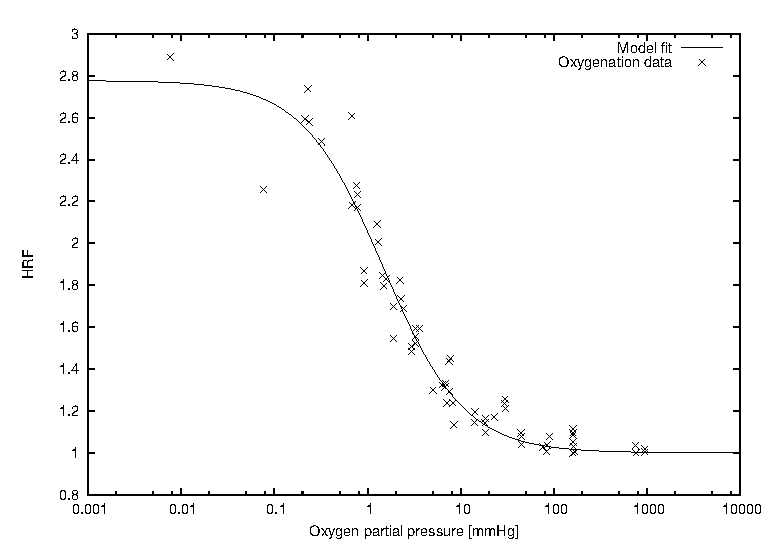
\includegraphics{/Users/alex/Master/contents/images/HRFModel.eps}
\caption{HRF model fit to original data from \textit{Carlson et al.}\cite{pmid21183291}. The new fit to the original data allowed an estimate on the error on $K$ and $m$ for the robustness analysis in the later part of this work.}
\label{fig:HRFModel}
\end{figure}
The model parameters $K$ and $m$ are generally unknown and have to be retrieved by fitting measured data. As HRF is basically built upon the same mathematical concept as OER, it is possible to reuse and transform measurements for OER. This can be done by dividing the maximum OER by the OER for each level of oxygenation. Table \ref{tab:modelparameter} gives an overview over all conducted searches for these model parameters and their respective mean values and standard deviations. The data from \textit{Carlson et al.}\cite{pmid21183291} have been reused to calculate the error on the fit, as it was not part of the publication. While the maximum HRF value $m$ value seem to be largely consistent to another, the $K$ value has a large spread. One of the reasons for these deviations is that all measurements conducted by \textit{Cullen et al.}\cite{pmid4616914, pmid1084867} are from the 1970s and exhibit larger errors in contrast to the measurement from  \textit{Carlson et al.}. The combined values for $K$ and $m$ in table \ref{tab:modelparameter} have been computed with a weighted mean to account for the large error differences in all presented measurements
\begin{equation}
\overline x = \frac{\sum\limits_{i=1}^n(x_i/\sigma_i^2)}{\sum\limits{i=1}^n(1/\sigma_i^2)}.
\end{equation}
The error on the combined value is the variance of the weighted mean of all measurements conducted
\begin{equation}
\sigma^2_{\overline x} = \frac{1}{\sum\limits_{i=1}^n(1/\sigma_i^2)}.
\end{equation}
The impact of HRF in radiotherapy can be derived by understanding its impact on the delivered biological effect. As the HRF decreases the radio response to radiation damage, the delivered effect becomes smaller as $\alpha$ and $\beta$ are scaled down. To compensate for this, either of two things have to done, to account for the decreased radio sensitivity:
\begin{enumerate}
\item Increase dose to a value, where the delivered effect with decreased radio sensitivity is equal to the prescribed effect under aerobic conditions. The dose $D$ to compensate for hypoxia can be calculate in terms of prescribed effect $\varepsilon_P = \alpha_XD_p + \beta_XD_p^2$ and prescribed dose $D_p$ (cf. Appendix \ref{appendix:a} for derivation)
\begin{equation}\label{eq:dosecompensation}
D = \mathrm{HRF}\left[\sqrt{\left(\frac{\alpha_X}{2\beta_X}\right)^2 + \frac{\varepsilon_p}{\beta_X}}-\frac{\alpha_X}{2\beta_X}\right].
\end{equation}
The dose is linearly scaled to the HRF within a voxel. If the usual prescription in a voxel is 70 Gy, a HRF of 2 implies that 140 Gy are necessary to create the same biological effect in this hypoxic area. As seen in table \ref{tab:modelparameter}, the maximum HRF is $m=2.82\pm 0.05$. Therefore in fully hypoxic areas with $p=0$ mmHg, the dose has to be increased with a factor of 2.82.
\item Administrate radio sensitizers to compensate for the decreased radio sensitivity. The effect on the biological effect can be summarized into the sensitizer enhancement ratio (SER). SER is dependent on the drug concentration $c$ and the current oxygen partial pressure $p(r)$, while the survival then reads as \cite{pmid21183291}
\begin{equation}
S(D) = \exp\left(\frac{\alpha_A\cdot\mathrm{SER}}{\mathrm{HRF}}D + \frac{\beta_A\cdot\mathrm{SER}^2}{\mathrm{HRF}^2}D^2\right).
\end{equation}
The administration of radio sensitizers is not part of this work, but should be considered as another way of decreasing the radio desensitization of tumour cells via acute and chronic hypoxia. If general dose painting should not prove feasible due to high dose fractions induced by hypoxia, radio sensitizers can decrease the effects this mechanism.
\end{enumerate}
\subsection{Assessment of chronic and acute hypoxia}\label{chapt:chronicacute}
As mentioned in chapter \ref{chap:hypoxiaorigin}, hypoxia can be categorized into chronic and acute hypoxia. Inclusion of acute hypoxia can lead to overestimation of hypoxia since it is transient and is is subject to temporal variance. To quantify the fractions of chronic and acute hypoxia \textit{Wang et al.} \cite{pmid19928070} proposed a model based on the SUV. The model assumes that both hypoxia types contribute to the total tracer uptake $H$
\begin{equation}
\mathrm{H} = \mathrm{H}_\mathrm{a} + \mathrm{H}_\mathrm{c},
\end{equation}
where $ \mathrm{H}_\mathrm{a}$ is the contribution of the acute and $ \mathrm{H}_\mathrm{c}$ of the chronic hypoxia to the tracer uptake. To distinguish two hypoxia types with the Wang model, it is necessary to analyze two functional images (such as positron emission tomography, cf. \ref{chapter:3}) of the same patient. This is due to the fact that only acute hypoxia shows a large temporal variance, while chronic hypoxia is seen as a constant. The total uptake in two functional images is
\begin{equation}
\mathrm{H}_i = \mathrm{H}_\mathrm{a,i} + \mathrm{H}_\mathrm{c} \hspace{0.5cm}\mathrm{for}\hspace{0.5cm}i=1,2
\end{equation}
Afterwards, all uptake values in the same voxels from the two functional images are sorted into high H$_\mathrm{h}$ and small H$_\mathrm{s}$ readings. The fraction of high uptakes H$_\mathrm{h}$ with respect to acute hypoxia is denoted $\omega = \mathrm{H}_\mathrm{ah}/\mathrm{H}_\mathrm{h}$. Defining $x = (\mathrm{H}_\mathrm{h} - \mathrm{H}_\mathrm{s})/\mathrm{H}_\mathrm{h}$ gives the following relation
\begin{equation}
\omega = \rho x^\beta,
\end{equation}
where $\beta=0.6$ is derived via Monte-Carlo simulation and $\rho$ can be calculated via an iterative best fit to a Gaussian distribution. For voxels that have high readings H$_\mathrm{h}$, the chronic contribution can be calculated via
\begin{equation}
\mathrm{H}_\mathrm{c} = (1-\rho x^\beta)\mathrm{H}_\mathrm{h}.
\end{equation}
\section{Treatment planning}
\subsection{Dose delivery with IMRT}
All treatment plans presented in this work are intensity modulated radiotherapy (IMRT) plans. IMRT has been proposed by Brahme \textit{et al} in 1982 \cite{pmid7146095}, while the clinical solution to the inverse IMRT optimization problem has been formulated by Webb in 1989 \cite{pmid2682694} inferring the minimization of a objective function via simulated annealing. The form of the objective function can differ in different treatment planning systems. Generally, objective functions are quadratic and describe the difference between a desired dose in a voxel from a dose prescription and the current dose calculated in the optimization step. Chapter \ref{chap:objectivefunctions} describes in more detail, how \textit{KonRad} implements such an objective function for physical dose and biological effect optimizations. Due to the physical nature of the optimization problem, the quadratic function does not have a local minimum, which allowed the implementation of a fast gradient approach to find the minimum instead \cite{pmid2243845}. The delivery of IMRT has been shown by Convery and Rosenbloom in 1992 \cite{Convery_Rosebloom_1992}, which was later used for MLC based IMRT treatment \cite{pmid8690638}. \\The intensity modulation achieved in IMRT can only be accomplished laterally to the the incident beam direction for photons. For protons and heavy ions, the finite range of particles allows a three dimensional variation of the intensity modulation \cite{pmid10071883}, also referred to as 3D IMPT.
\subsection{Treament planning with \textit{KonRad}}
All treatment plans in this work are optimized using the treatment planning system \textit{KonRad} \cite{nill}. \textit{KonRad} is able to optimize treatment plans with carbon ions, protons, photons, electrons. It is also possible to create a combination of those modalities into one treatment plan. The basis of \textit{KonRad}'s plan optimization is a dose matrix $D_{ij}$. It describes the dose that a doseburst $j$ deposits in voxel $i$ for a unity fluence. A doseburst can be described as the smallest field element that can be varied. In case of photons this is the smallest opening of an multi-leaf collimator (MLC). The dose $D_i$ in voxel $i$ is dependent on the number of dosebursts $N_{\mathrm{DB}}$
\begin{equation}
D_i = \sum\limits_{j=1}^{N\mathrm{DB}}D_{ij}w_j.
\end{equation}
$w_j$ is the weight of the doseburst $j$, while $D_{ij}$ is the dose matrix described earlier. With the implementation of the dose matrix $D_{ij}$ in \textit{KonRad} it is possible to separate dose calculation from the optimization process. This enables \textit{KonRad} to speed up the optimization process, since the dose needs no recalculation after each optimization step. While $D_{ij}$ describes the physical dose, \textit{KonRad} has been modified to calculate biological effect for carbon ions \cite{pmid16757867} and protons \cite{pmid15285249}, as well as for Intensity Modulated Proton Therapy (IMPT) \cite{pmid15789592}. The optimization process in \textit{KonRad} for IMRT uses the LBFGS-B code \cite{Byrd_Lu_Nocedal_Zhu_1994} as the quasi-Newton approach for the minimization of the objective function.
\subsection{Physical Objective function}\label{chap:objectivefunctions}
Treatment planning with biological dose painting is implemented into the treatment planning system KonRad \cite{nill}. The optimization in Konrad minimizes an objective function $F$ that is defined as the weighted sum of the objective functions for each volume
\begin{equation}
F(\mathbf{w}) = \sum\limits_{v\in\mathrm{Targets}}\left(p_v^UF_v^U(\mathbf{w}+p_v^OF_v^O(\mathbf{w})\right) + \sum\limits_{v\in\mathrm{OAR}}p_v^OF_v^O(\mathbf{w}).
\end{equation}
Here $\mathbf{w}$ is the vector of the weights defining the fluence of each the dosebursts. The quadratic objective function for each target and each OAR are weighted with individual penalty factors $p_v$ that can be defined independently for underdose ($p^U$) and overdosage ($p^O$). The physical objective function for a volume $v$ is given by \cite{pmid11444513}
\begin{equation}
F_v^O (\mathbf{w}) = \sum\limits_{i\in v} \left|D_i(\mathbf{w})-\overline{D}_v^O\right|_+^2\hspace{1cm}F_v^U (\mathbf{w}) = \sum\limits_{i\in v} \left|\overline{D}_v^U-D_i(\mathbf{w})\right|_+^2
\end{equation}
where $\overline{D}_v$ is the respective prescribed absorbed dose for volume $v$. The dose $D_i(\mathbf{w})$ is the calculated dose according to
\begin{equation}
D_i(\mathbf{w}) = \sum\limits_{j=1}^{N_{\mathrm{DB}}} D_{ij}w_j,
\end{equation}
with $D_{ij}$ being the dose matrix, and $N_{\mathrm{DB}}$ the number of dosebursts. The function $|x|_+$ is defined as 0 for $x\leq0$ and $x$ if $x>0$.
\subsection{Dose calculation \& biological effect}
Before the optimization, the dose matrix $D_{ij}$ has to be calculated. This calculate has to be executed for every bixel $j$ and voxel $i$. \textit{KonRad} uses a finite pencil beam dose calculation model\cite{nill}. To account for biological properties in the biological optimization, the $D_{ij}$ approach has been extended in this work. As the biological effect depends on the radio response parameters $\alpha$ and $\beta$ is it useful to introduce matrices. Due to mathematical reasons (cf. equation \ref{eq:betadose}) it is important to store the square-root of the $\beta_i$ in the $\beta_{ij}$ matrix. This is due to the physical nature of radiation superimposition: If more than one doseburst hits a voxel $i$ one needs to superimpose the effects of the radiation. For the radio response parameters $\alpha$ and $\beta$ the superimposition can be calculate in the following way \cite{pmid7413933} \cite{pmid16757867}
\begin{equation}\label{eq:betadose}
\alpha = \frac{1}{D}\sum\limits_{i=1}^N\alpha_i D\hspace{1cm}\sqrt{\beta} = \frac{1}{D}\sum\limits_{i=1}^N\sqrt{\beta_i}D_i.
\end{equation}
By combing the synergistic effects from different dosebursts in biological optimization the total biological effect in voxel $i$ is given by \cite{pmid16757867}
\begin{equation}
\varepsilon_i(\mathbf{w}) = \sum\limits_{j=1}^N\alpha_{ij}D_{ij}w_j+\left(\sum\limits_{j=1}^N\sqrt{\beta_{ij}}D_{ij}w_j\right)^2.
\end{equation}
Therefore the biological objective function is proportional to $\mathbf{w}^4$. Due to the nature of the higher order of the optimization function it is possible that in some cases the biological objective function is not convex\cite{FreseThesis}.
\subsection{Biological objective function}
To implement biological effect optimization, KonRad can be altered by introducing the biological effect $\varepsilon = \alpha D + \beta D^2$ into the physical optimization function. The quadratic difference between the prescribed effect $\overline{\varepsilon}_v$ and the actual effect $\varepsilon_i(\mathbf{w})$ is minimized using the same approach \cite{FreseThesis}:
\begin{equation}
F_v^O (\mathbf{w}) = \sum\limits_{i\in v} \left|\varepsilon_i(\mathbf{w})-\overline{\varepsilon}_v^O\right|_+^2\hspace{1cm}F_v^U (\mathbf{w}) = \sum\limits_{i\in v} \left|\overline{\varepsilon}_v^U-\varepsilon_i(\mathbf{w})\right|_+^2
\end{equation}
For each doseburst $j$ that deposit a dose $D_{ij}w_j$ in the voxel $i$ it is necessary to calculate the linear quadratic model parameters $\alpha_{ij}$ and $\beta_{ij}$.
